Ne interesează să găsim \textit{cea mai bună strategie}. Pentru a compara între ele mai multe strategii, trebuie să gândim \textit{un mediu în care acestea să concureze}. 
 
Până la a găsi cea mai bună strategie, trebuie, mai întâi, să vedem cum anume poate configurația unui algoritm genetic să influențeze calitatea soluției. De asemenea, vrem să vedem cum anume se comportă într-un mediu de test strategia propusă de algoritm. 
 
Pentru a îndeplini aceste cerințe, am ales să supun cromozomii la un anumit tip de turneu, ce poartă denumirea de \textbf{turneu cu eliminare}.  

\section {Termeni întâlniţi}
O \textbf{rundă} este dată de alegerea, în mod secret, a mișcării următoare și actualizarea scorului în funcție de ce a pus și oponentul. 

Un \textbf{meci} este jucat de către doi jucători. Este alcătuit dintr-un număr de runde. În fiecare rundă, fiecare jucător alege, în mod secret, ce mișcare va face. La final de rundă, scorul jucătorilor este actualizat cu o valoare dată de mișcarea făcută de fiecare, în funcție de ce a ales și oponentul să facă. 

\section {Cum este modelat un turneu cu eliminare}
 
Un turneu cu eliminare pornește de la o populație de strategii în care, la fiecare iterație, fiecare individ joacă câte un meci cu ceilalți indivizi. Pe parcursul meciurilor, câștigurile individuale se însumează într-un scor total. După ce se joacă toate combinările de doi jucători (se ajunge la finalul iterației), se elimină un procent din cei mai slabi jucători.  Pentru a mai reduce din numărul parametrilor ale căror valori pot varia, am stabilit că procentul să fie de 25\%. În caz de egalitate a scorurilor între doi jucători, se elimină la întâmplare unul din cei doi. Se completează locurile eliberate cu stategii care au obținut printre cele mai bune scoruri. Se resetează scorul total al indivizilor și se repetă acești pași până când în turneu a rămas un singur tip de strategie, ori până când am atins un număr maxim de iterații.  
\\\\
\textit{Observație}: Când într-un turneu cu eliminare concurează doi indivizi ce au aceeași strategie deterministă, la finalul unei iterații, cei doi indivizi vor avea exact același scor. Nu putem spune același lucru despre doi indivizi care folosesc strategia \textbf{Random}.
\\\\
Pentru a vedea clar modul în care evoluează strategiile în contextul acestui tip de turneu, am implementat o metodă grafică de vizualizare a datelor. Am ales să folosesc \textbf{line chart}-uri. Axa absciselor are drept legendă numărul de indivizi din fiecare strategie. Axa ordonatelor reprezintă indexul rundei turneului.

\section {Concluzii trase în urma finalizării turneelor}

Fiecare experiment este dat de stabilirea parametrilor configurației algoritmului genetic, urmată de rularea algoritmului genetic și trecerea soluției prin mai multe medii de testare, prin varierea configurației turneului cu eliminare.

În contextul acestei probleme, nu putem vorbi despre optim local sau global, întrucât un fitness cu o valoare bună obținut pentru un cromozom în faza de antrenare poate să își piardă relevanța în faza de testare datorită faptului că mediul de testare poate varia. 

În rândurile următoare prezint o serie de experimente.  

\subsection {Explorarea redusă a spațiului de căutare} 

\begin{center}
	\underline{\textit{Experimentul 1}}
\end{center}

\textit{Configurația algoritmului genetic și cea a turneului cu eliminare este trecută în \textbf{Anexa numărul 1}}.\\

Am făcut un prim experiment în care configurația algoritmului genetic a dus la o explorare redusă a spațiului de căutare. Pentru aceasta, am ales valori mici pentru numărul de generații, pentru numărul de runde din turneul clasic și pentru probabilitățile operatorilor genetici.
 
Diagramele de mai jos atestă calitatea redusă a soluției obținute în urma experimentului. 

\begin{figure}[H]
	\centering
	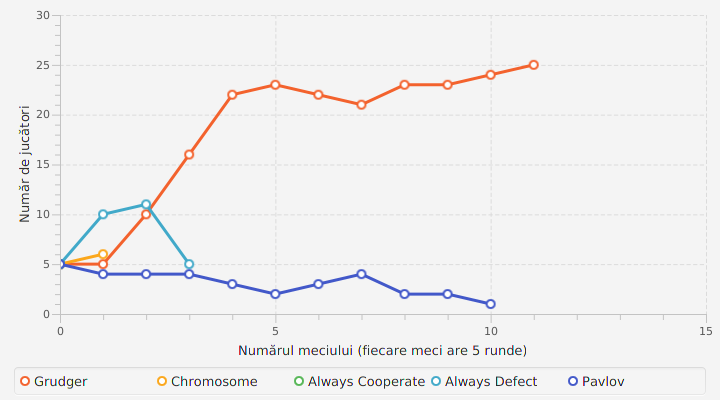
\includegraphics[	
	width=16cm,
	height=7.5cm,
	keepaspectratio
	]{imagini/experiment_1_epoch_1529303072346/chart_from_epoch_1529303304972.png}
	\caption{}
\end{figure}

\begin{figure}[H]
	\centering
	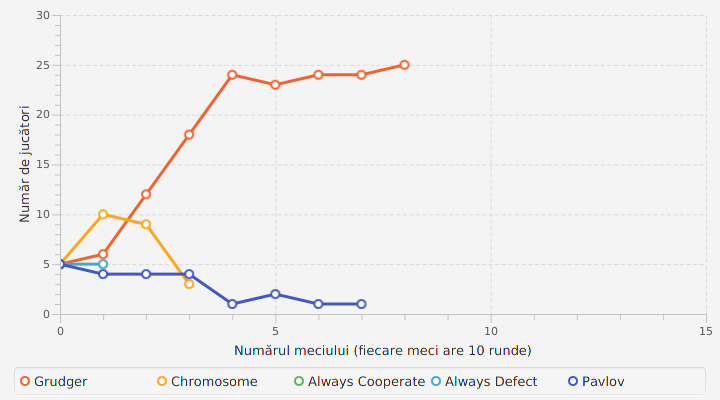
\includegraphics[	
	width=16cm,
	height=7.5cm,
	keepaspectratio
	]{imagini/experiment_1_epoch_1529303072346/chart_from_epoch_1529303340019.png}
	\caption{}
\end{figure}

\begin{figure}[H]
	\centering
	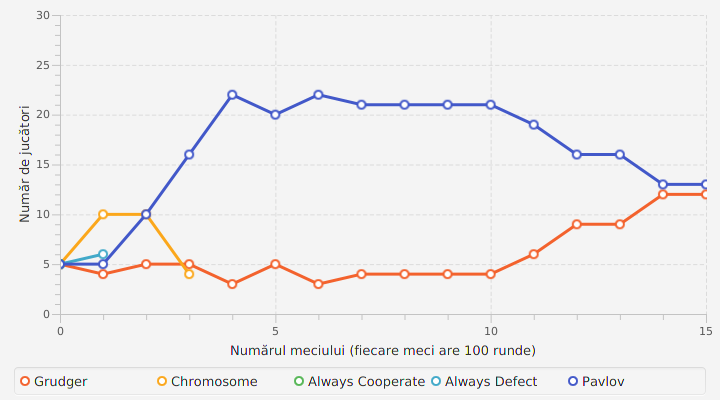
\includegraphics[	
	width=16cm,
	height=7.5cm,
	keepaspectratio
	]{imagini/experiment_1_epoch_1529303072346/chart_from_epoch_1529303352244.png}
	\caption{}
\end{figure}

\begin{figure}[H]
	\centering
	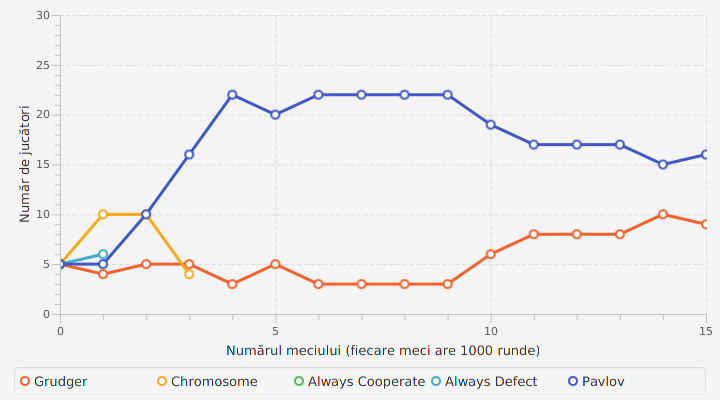
\includegraphics[	
	width=16cm,
	height=7.5cm,
	keepaspectratio
	]{imagini/experiment_1_epoch_1529303072346/chart_from_epoch_1529303371162.png}
	\caption{}
\end{figure}

\subsection {Numărul de runde al meciurilor din turneul cu eliminare}

\begin{center}
	\underline{\textit{Experimentul 2}}
\end{center}

\textit{Configurația algoritmului genetic și cea a turneului cu eliminare este trecută în \textbf{Anexa numărul 2}}.\\

Într-un alt experiment, am surpins cum numărul de runde, odată modificat cu o valoare foarte mică, a avantajat una din strategiile algoritmului genetic. 

\begin{figure}[H]
	\centering
	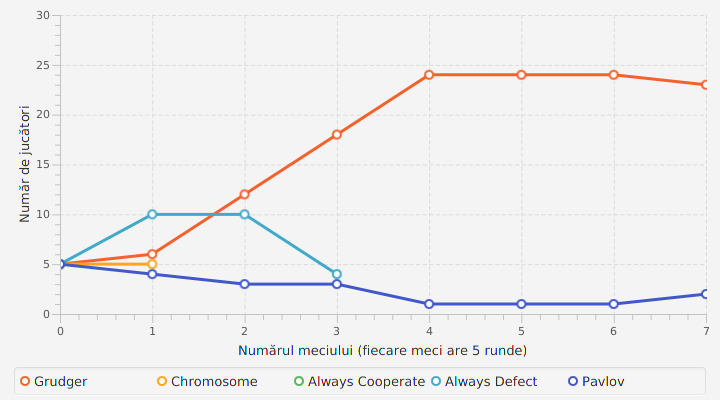
\includegraphics[	
	width=16cm,
	height=7.5cm,
	keepaspectratio
	]{imagini/experiment_2_epoch_1529309949939/chart_from_epoch_1529310422567.png}
	\caption{}
\end{figure}

\begin{figure}[H]
	\centering
	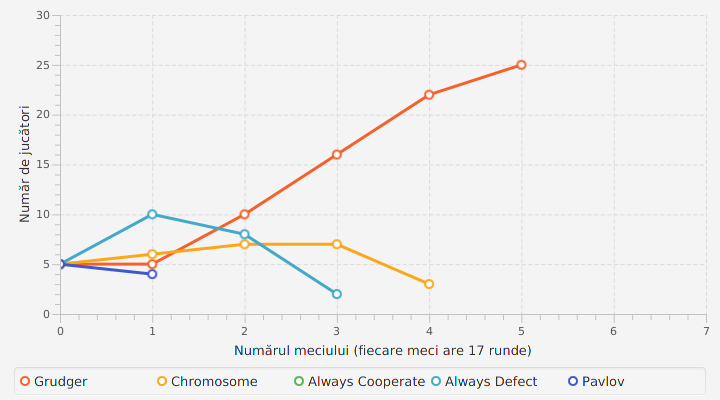
\includegraphics[	
		width=16cm,
		height=7.5cm,
		keepaspectratio
	]{imagini/experiment_2_epoch_1529309949939/chart_from_epoch_1529310399495.png}
	\caption{}
\end{figure}

Mărind cu 1 numărul de runde din fiecare meci, observăm că strategia propusă de algoritmul genetic câștigă. 

\begin{figure}[H]
	\centering
	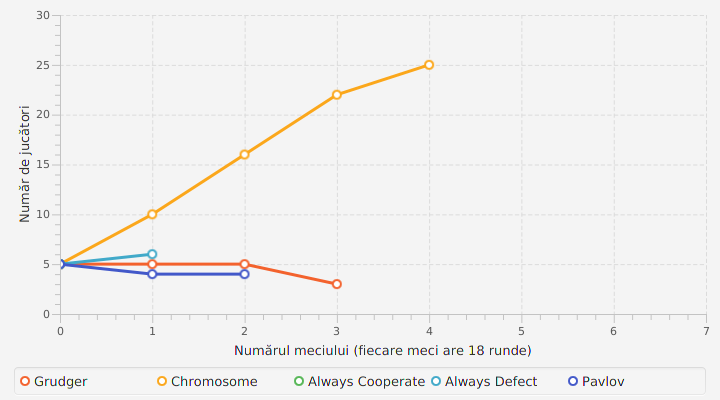
\includegraphics[	
	width=16cm,
	height=7.5cm,
	keepaspectratio
	]{imagini/experiment_2_epoch_1529309949939/chart_from_epoch_1529310386663.png}
	\caption{}
\end{figure}

\subsection{Strategia \textbf{Random}}

\begin{center}
	\underline{\textit{Experimentele 3 și 4}}
\end{center}

\textit{Configurația algoritmului genetic și cea a turneului cu eliminare este trecută în \textbf{Anexa numărul 3}}.\\
 
Strategia \textbf{Random} nu reprezintă o problemă pentru strategiile oferite de algoritmul genetic.

Am antrenat o populație de dimensiune mică într-un număr mare de generații, lansând valori mari ale mutației și încrucișării. Populația de antrenament este dată de un singur individ de tip \textbf{Random}. Am rulat două experimente în urma cărora am obținut două strategii: pentru prima strategie obținută, cea din experimentul numărul 3, numărul de runde al tuneului clasic este mai mic (5 runde). Pentru celălalt experiment, numărul de runde al turneului clasic este 100.

\begin{figure}[H]
	\centering
	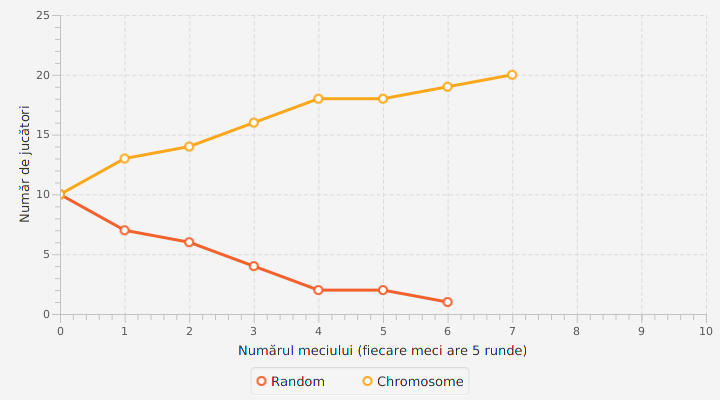
\includegraphics[	
	width=16cm,
	height=7.5cm,
	keepaspectratio
	]{imagini/experiment_3_epoch_1529321586156/chart_from_epoch_1529323404815.png}
	\caption{Cromozomii au strategia de la experimentul 3}
\end{figure}

\begin{figure}[H]
	\centering
	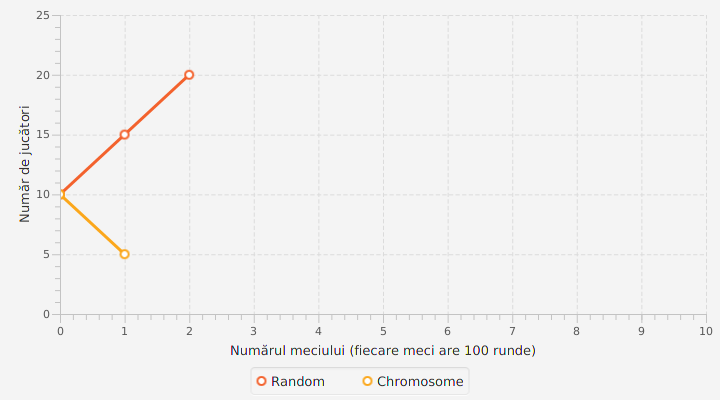
\includegraphics[	
	width=16cm,
	height=7.5cm,
	keepaspectratio
	]{imagini/experiment_3_epoch_1529321586156/chart_from_epoch_1529323424012.png}
	\caption{Cromozomii au strategia de la experimentul 3}
	\label{pierde_cromozomul_castiga_random}
\end{figure}

În Figura \ref{pierde_cromozomul_castiga_random}, se observă cum strategia propusă de algoritmul genetic pierde, întrucât nu este optimizată pentru a câștiga în contextul unui turneu cu număr mare de runde. 

\begin{figure}[H]
	\centering
	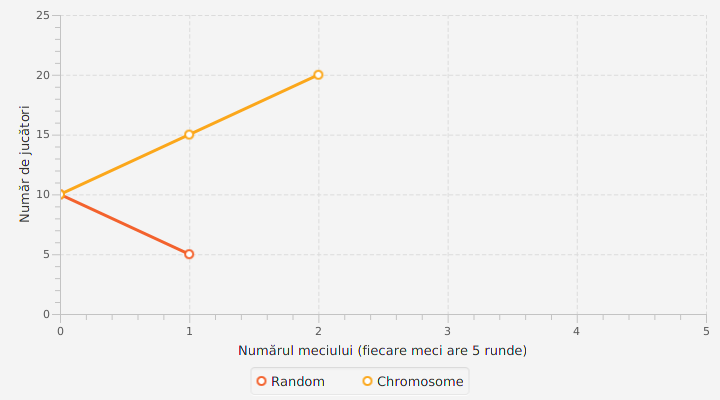
\includegraphics[	
	width=16cm,
	height=7.5cm,
	keepaspectratio
	]{imagini/experiment_4_epoch_1529323027289/chart_from_epoch_1529323309315.png}
	\caption{Cromozomii au strategia de la experimentul 4}
\end{figure}

\begin{figure}[H]
	\centering
	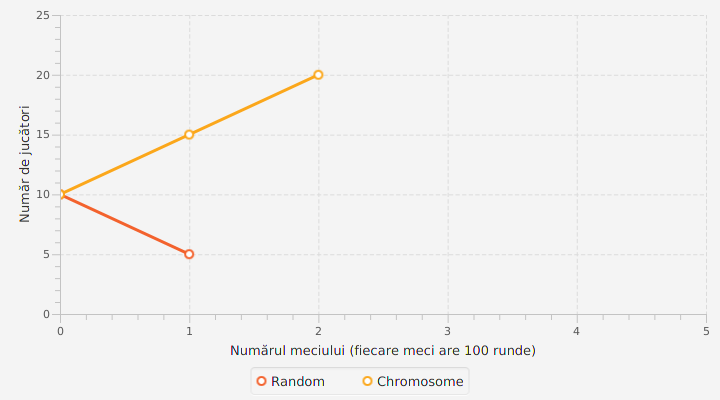
\includegraphics[	
	width=16cm,
	height=7.5cm,
	keepaspectratio
	]{imagini/experiment_4_epoch_1529323027289/chart_from_epoch_1529323321406.png}
	\caption{Cromozomii au strategia de la experimentul 4}
\end{figure}

Strategia din experimentul cu numărul 4 va face față și la un număr de runde mai mic, dar și la un număr de runde mai mare în turneele cu eliminare în fața strategiei \textbf{Random}. În fața acestei configurații a turneului eliminatoriu, putem trage concluzia că experimentul numărul 4 oferă o soluție mai bună. 

\subsection{Strategia Tit-For-Tat}

Un lucru ce se observă ușor este că strategia \textbf{Tit-For-Tat} reușește să câștige aproape de fiecare dată când la initiaizarea turneului cu eliminare toate strategiile au ponderi egale si numarul de runde este mare.

Se observa o limitare in ceea ce priveste cautarea unei configuratii a agoritmului genetic care sa ofere un oponent bun pentru Tit-For-Tat. Am facut un experiment in care populatia de antrenament este data de un individ cu strategia Tit-For-Tat, insa nu am obtinut rezultate bune. Cand concurau doar copii ale cromozomilor si copii ale strategiei Tit-For-Tat in proportii agele, de fiecare data, la pasii eliminatorii, se eliminau cromozomii.
 
  
Strategia Tit-For-Tat poate fi batuta doar daca schimbam configuratia turneului cu eliminare. Avem nevoie de un numar mic de runde si de o str




















































































































































































































